\documentclass{article}
\usepackage[utf8]{inputenc}
\usepackage{hyperref}
\usepackage{listings}
\usepackage{multimedia} % to embed movies in the PDF file
\usepackage{graphicx}
\usepackage{comment}
\usepackage[english]{babel}
\usepackage{amsmath}
\usepackage{amsfonts}
\usepackage{wrapfig}
\usepackage{multirow}
\usepackage{verbatim}
\usepackage{float}
\usepackage{cancel}
\usepackage{caption}
\usepackage{subcaption}
\usepackage{mathdots}
\usepackage{/home/cade/Homework/latex-defs}


\title{AMATH 574 Homework 2}
\author{Cade Ballew \#2120804}
\date{January 26, 2023}

\begin{document}
	
\maketitle
	
\section{Problem 3.4}
Consider the acoustics equations (3.30) 
\[
\begin{pmatrix}
	p\\u
\end{pmatrix}_t+A\begin{pmatrix}
p\\u
\end{pmatrix}_x
\]
with
\[
A=\begin{pmatrix}
	0 &K_0\\1/\rho_0 &0
\end{pmatrix},\quad \mathring p(x)=\begin{cases}
1,&1\leq x\leq2,\\
0,&\text{otherwise},
\end{cases},\quad\mathring u(x)=0.
\]
From chapter 2, we have that the eigenpairs of $A$ are given by $\lambda^1=-c_0$, $\lambda^2=c_0$ and
\[
r^1=\begin{pmatrix}
	-Z_0\\1
\end{pmatrix},\quad r^2=\begin{pmatrix}
Z_0\\1
\end{pmatrix}
\]
where $c_0=\sqrt{K_0/\rho_0}$ and $Z_0=\rho_0c_0$. Following the procedure for solving a Cauchy problem, we compute
\begin{align*}
\mathring{w}(x)=R^{-1}\mathring{q}=\frac{1}{2}\begin{pmatrix}
	u_0(x)-p_0(x)/Z_0\\
	u_0(x)+p_0(x)/Z_0
\end{pmatrix}
\end{align*} 
using Mathematica. We then use Mathematica to compute 
\begin{align*}
q(x,t)&=\mathring{w}^1(x+c_0t)\begin{pmatrix}
	-Z_0\\1
\end{pmatrix}+\mathring{w}^2(x-c_0t)\begin{pmatrix}
	Z_0\\1
\end{pmatrix}\\&=
\frac{1}{2}\begin{pmatrix}
p_0(x-c_0t)+p_0(x+c_0t)+Z_0(u_0(x-c_0t)-u_0(x+c_0t))\\
\frac{1}{Z_0}(p_0(x-c_0t)-p_0(x+c_0t))+u_0(x-c_0t)+u_0(x+c_0t)
\end{pmatrix}
\end{align*}
which is a general solution to this equation with $u_0=0$. Plugging in our initial data for this problem and noting that we're solving for $t>0$, we get that
\begin{align*}
q(x,t)&=\begin{pmatrix}
	p_0(x-c_0t)+p_0(x+c_0t)\\
	\frac{1}{Z_0}(p_0(x-c_0t)-p_0(x+c_0t))
\end{pmatrix}\\&=
\begin{cases}
\begin{pmatrix}
	0\\0
\end{pmatrix}, &x+c_0t<1,x-c_0t>2,\text{ or }x-c_0t<1<2<x+c_0t,\\
\begin{pmatrix}
	\frac{1}{2}\\-\frac{1}{2Z_0}
\end{pmatrix}, &x-c_0t<1\leq x+c_0t\leq2,\\
\begin{pmatrix}
	1\\0
\end{pmatrix}, &1\leq x-c_0t\leq x+c_0t\leq2,\\
\begin{pmatrix}
	\frac{1}{2}\\\frac{1}{2Z_0}
\end{pmatrix}, &1\leq x-c_0t\leq2< x+c_0t
\end{cases}
\end{align*}
which depends piecewise on the characteristics. We include the following (crude) sketches of the solution in the $x$-$t$ plane and the $p$-$u$ phase plane.\\
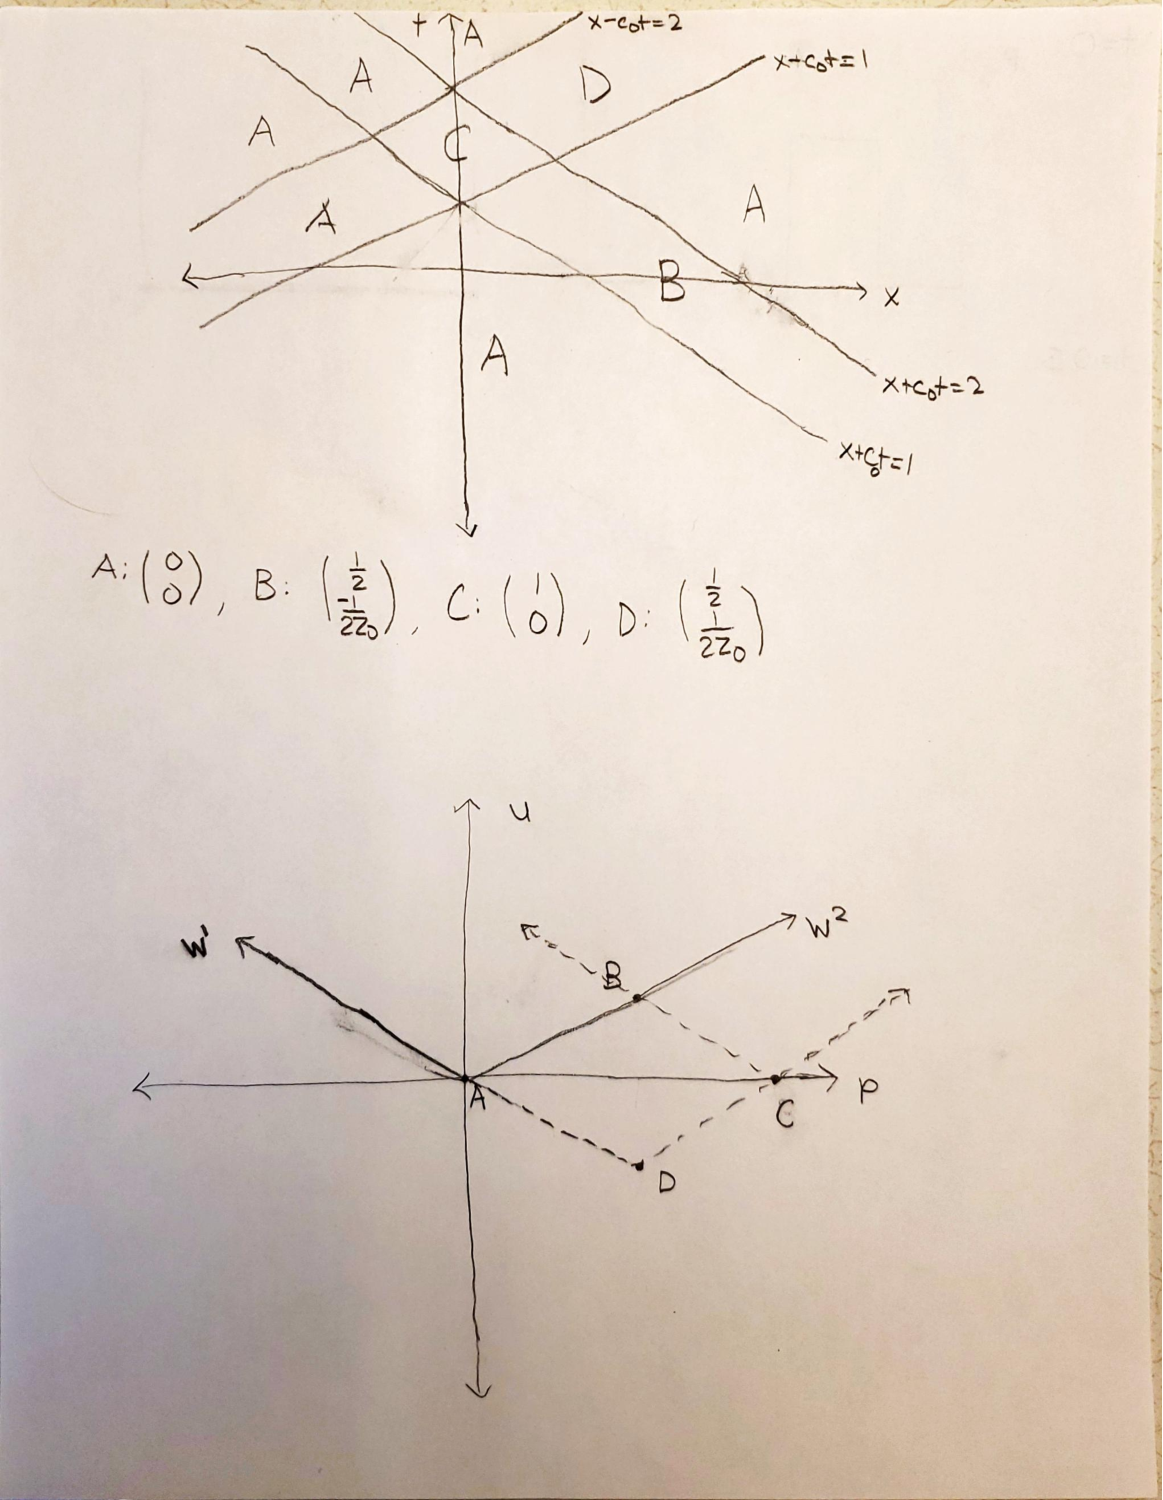
\includegraphics[scale=0.45]{574figs1v2.pdf}

\section{Problem 3.5}
Now, we wish to solve problem 3.4 on the finite domain $0\leq x\leq4$ with boundary conditions $u(0,t)=u(4,t)=0$. Following section 7.3.3, we do this by solving the Cauchy problem with our initial condition reflected across the boundaries. Namely, we consider
\[
\mathring p(x)=\begin{cases}
	1,&x\in[-2,-1]\cup[1,2]\cup[6,7],\\
	0,&\text{otherwise},
\end{cases},\quad\mathring u(x)=0.
\]
Letting $\mathcal A=[-2,1]\cup[1,2]\cup[6,7]$, our solution is now given by
\begin{align*}
	q(x,t)&=\begin{pmatrix}
		p_0(x-c_0t)+p_0(x+c_0t)\\
		\frac{1}{Z_0}(p_0(x-c_0t)-p_0(x+c_0t))
	\end{pmatrix}\\&=
	\begin{cases}
		\begin{pmatrix}
			0\\0
		\end{pmatrix}, &x+c_0t,x-c_0t\notin\mathcal{A},\\
		\begin{pmatrix}
			\frac{1}{2}\\-\frac{1}{2Z_0}
		\end{pmatrix}, &x-c_0t\notin\mathcal{A},~ x+c_0t\in\mathcal{A},\\
		\begin{pmatrix}
			1\\0
		\end{pmatrix}, &x+c_0t,x-c_0t\in\mathcal{A},\\
		\begin{pmatrix}
			\frac{1}{2}\\\frac{1}{2Z_0}
		\end{pmatrix}, &x-c_0t\in\mathcal{A},~ x+c_0t\notin\mathcal{A}.
	\end{cases}
\end{align*}
This solution now depends even more heavily on the characteristics in the manner of the following figure.\\
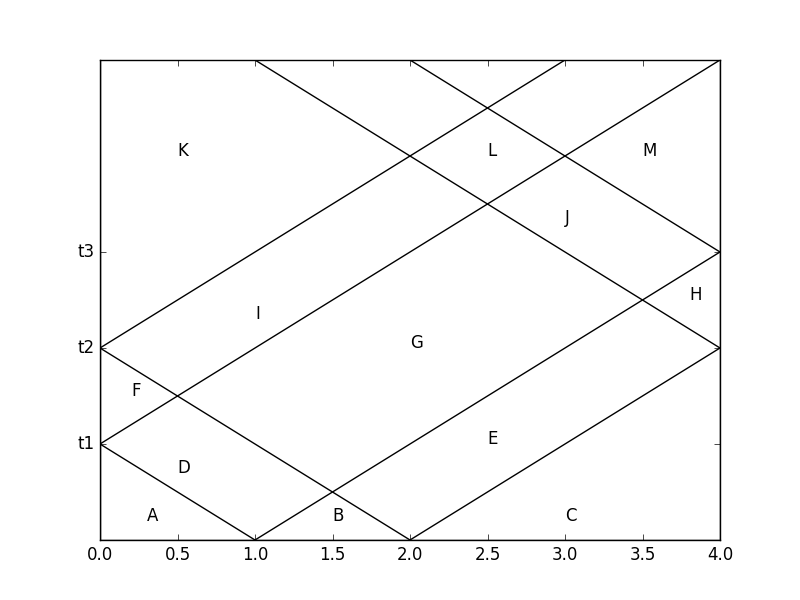
\includegraphics[scale=0.5]{problem_3_5.png}\\
We determine $t_1,t_2,t_3$ by finding where the characteristics intersect the boundaries. We consider $x\pm c_0t=a$ where $a$ is an endpoint of one of our intervals. On the left, we have $c_0t=1,2$, so $t_1=1/c_0$, $t_2=2/c_0$. On the right, we have $4+c_0t=6,7$, so $t_3=3/c_0$. Now, we use our piecewise solution to determine $A,\ldots,M$.
\begin{align*}
&A=\begin{pmatrix}
	0\\0
\end{pmatrix},\quad B=\begin{pmatrix}
1\\0
\end{pmatrix},\quad C=\begin{pmatrix}
0\\0
\end{pmatrix},\quad D=\begin{pmatrix}
\frac{1}{2}\\-\frac{1}{2Z_0}
\end{pmatrix},\quad E=\begin{pmatrix}
\frac{1}{2}\\\frac{1}{2Z_0}
\end{pmatrix},\\
&F=\begin{pmatrix}
1\\0
\end{pmatrix},\quad G=\begin{pmatrix}
	0\\0
\end{pmatrix},\quad H=\begin{pmatrix}
1\\0
\end{pmatrix},\quad I=\begin{pmatrix}
\frac{1}{2}\\\frac{1}{2Z_0}
\end{pmatrix},\quad J=\begin{pmatrix}
\frac{1}{2}\\-\frac{1}{2Z_0}
\end{pmatrix},\\
&K=\begin{pmatrix}
0\\0
\end{pmatrix},\quad L=\begin{pmatrix}
1\\0
\end{pmatrix},\quad M=\begin{pmatrix}
0\\0
\end{pmatrix}.
\end{align*}
Now, we include plots of $p(x,t),u(x,t)$ at times $t=0,0.5,1,1.5,2,3$ which were created in Julia with the parameter values $c_0=1$, $Z_0=0.7$.\\
\begin{figure}[H]
	\centering
	\begin{subfigure}{0.495\linewidth}
		\centering
		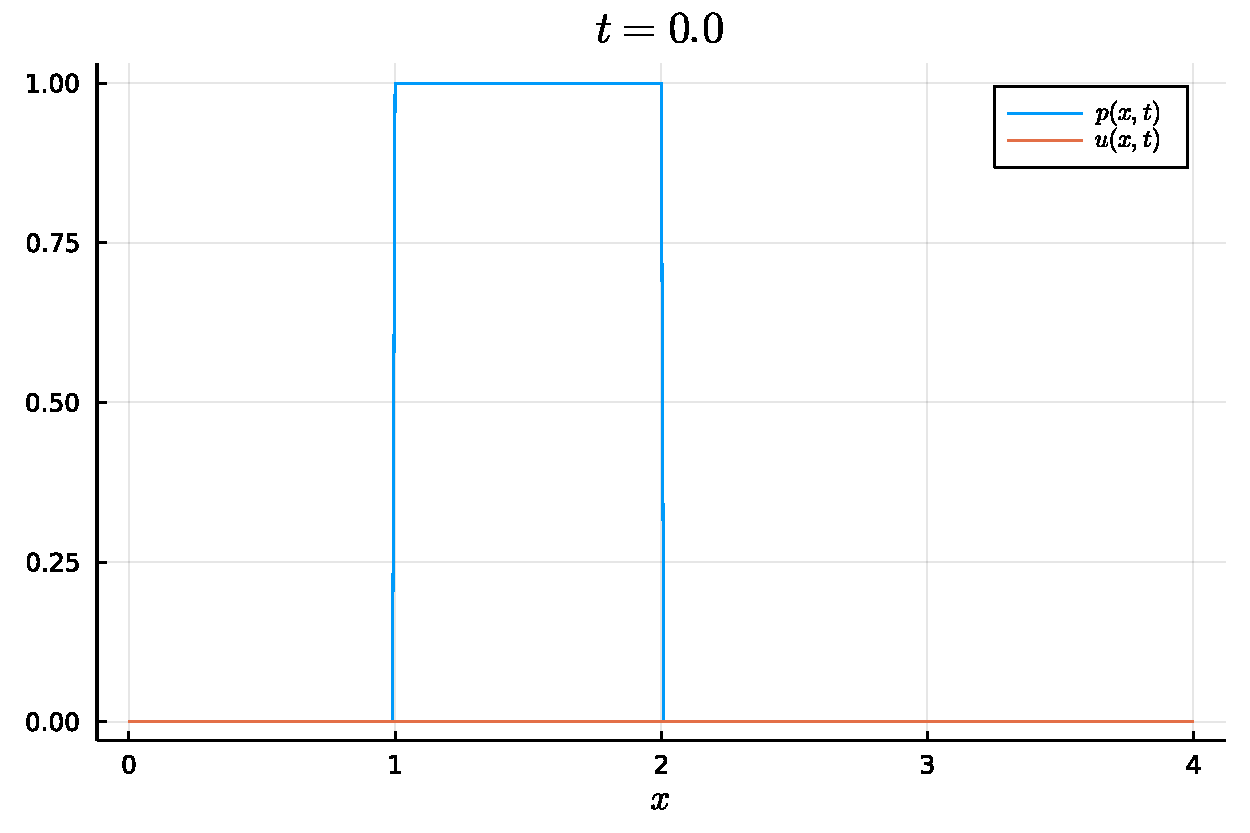
\includegraphics[width=\linewidth]{prob3-5-1.pdf}
	\end{subfigure}
	\begin{subfigure}{0.495\linewidth}
		\centering
		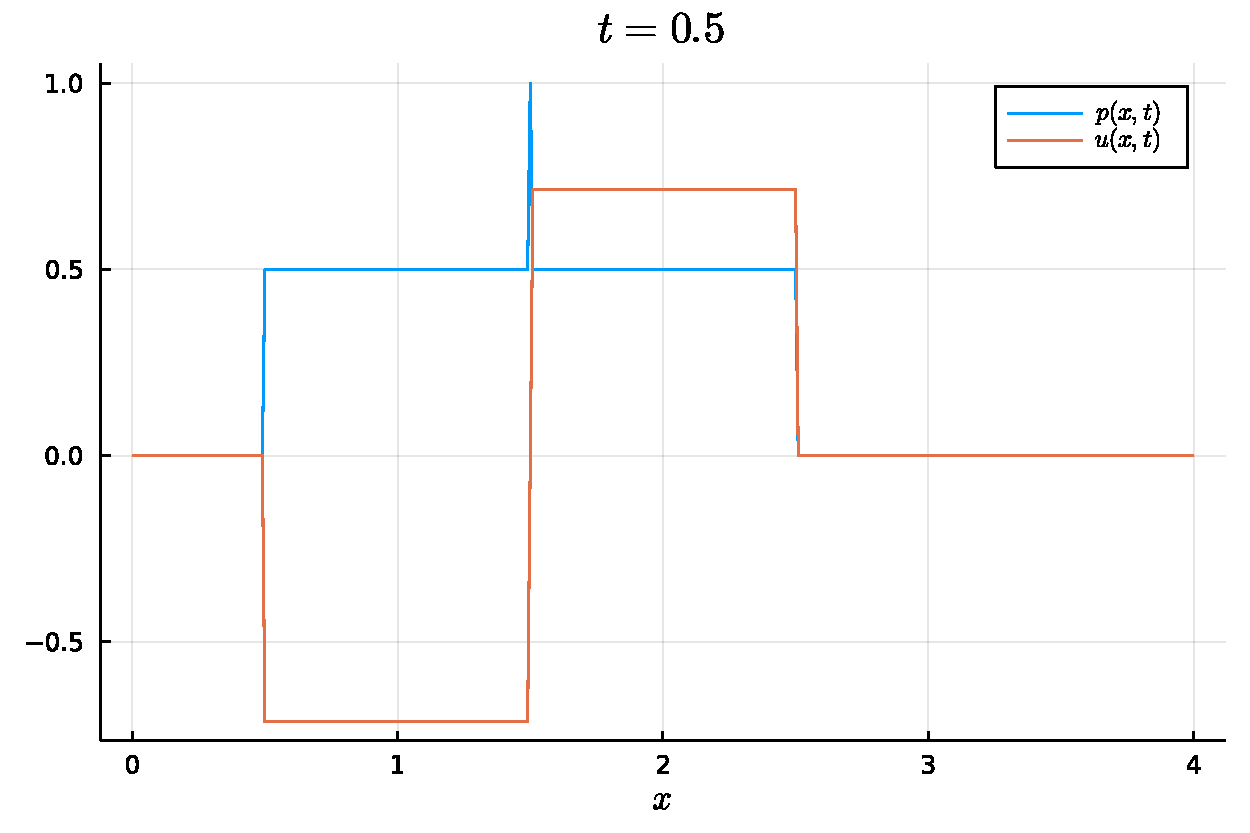
\includegraphics[width=\linewidth]{prob3-5-2.pdf}
	\end{subfigure}
	\begin{subfigure}{0.495\linewidth}
		\centering
		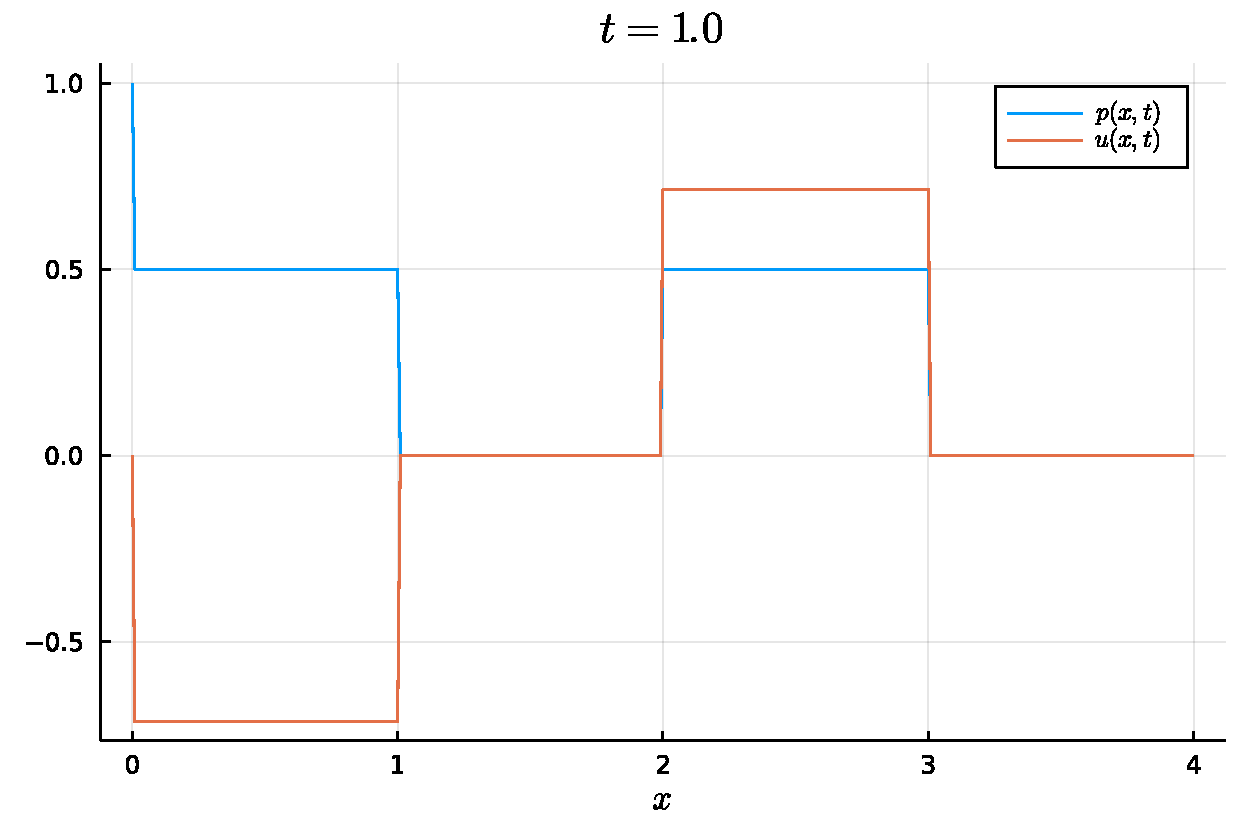
\includegraphics[width=\linewidth]{prob3-5-3.pdf}
	\end{subfigure}
	\begin{subfigure}{0.495\linewidth}
		\centering
		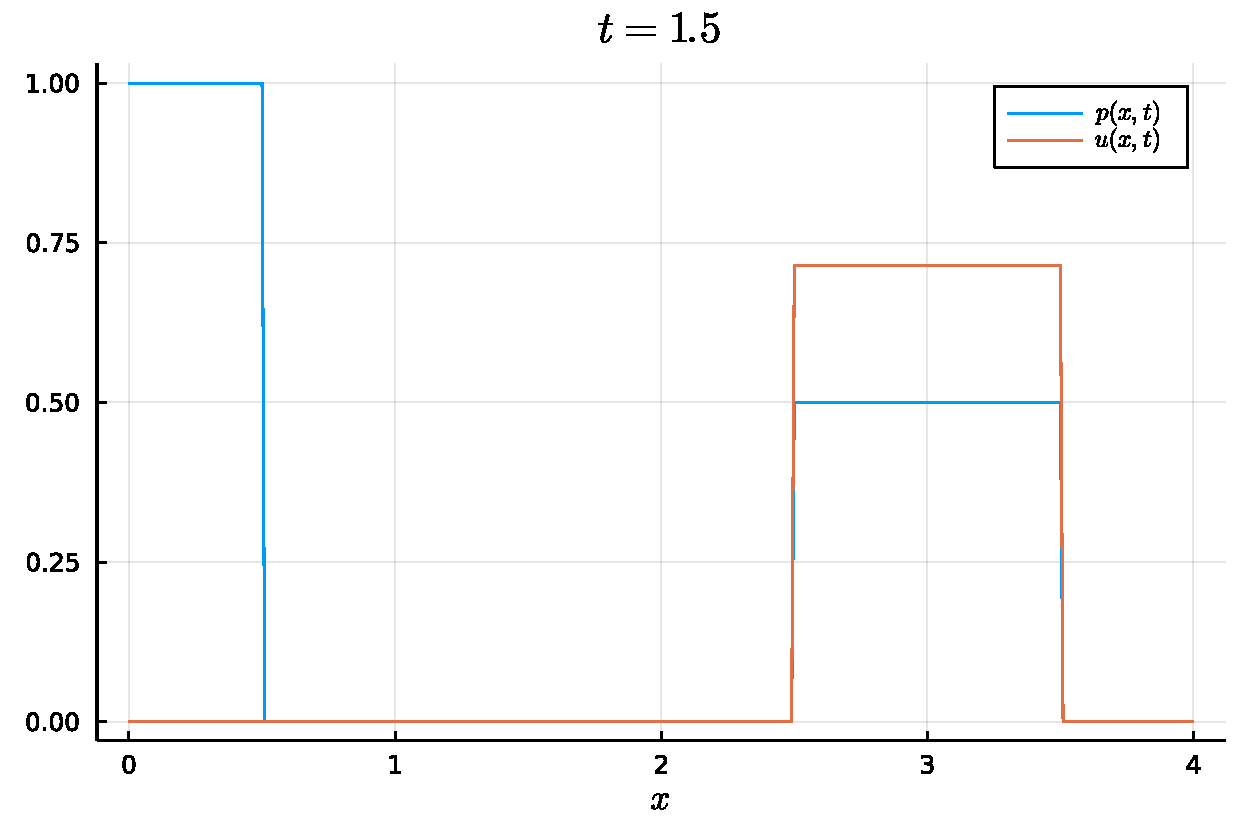
\includegraphics[width=\linewidth]{prob3-5-4.pdf}
	\end{subfigure}
	\begin{subfigure}{0.495\linewidth}
	\centering
	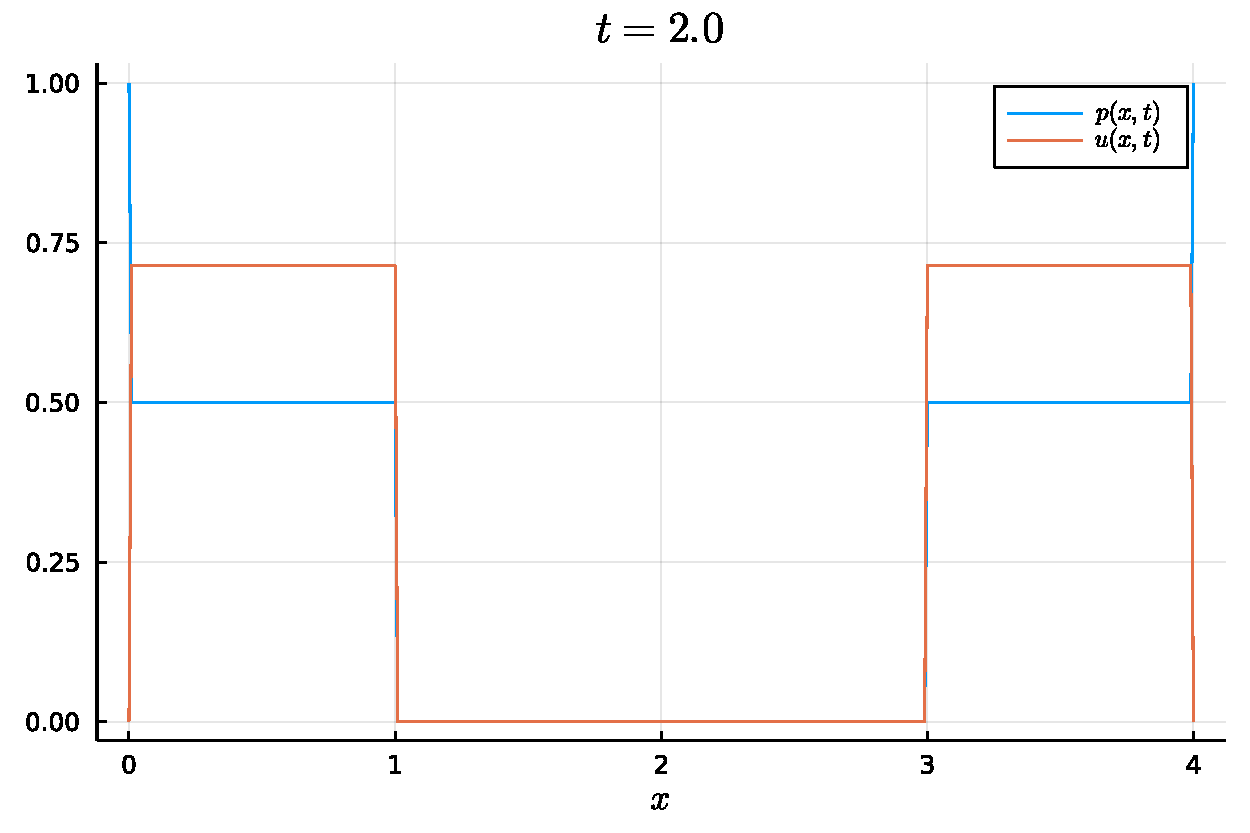
\includegraphics[width=\linewidth]{prob3-5-5.pdf}
\end{subfigure}
	\begin{subfigure}{0.495\linewidth}
	\centering
	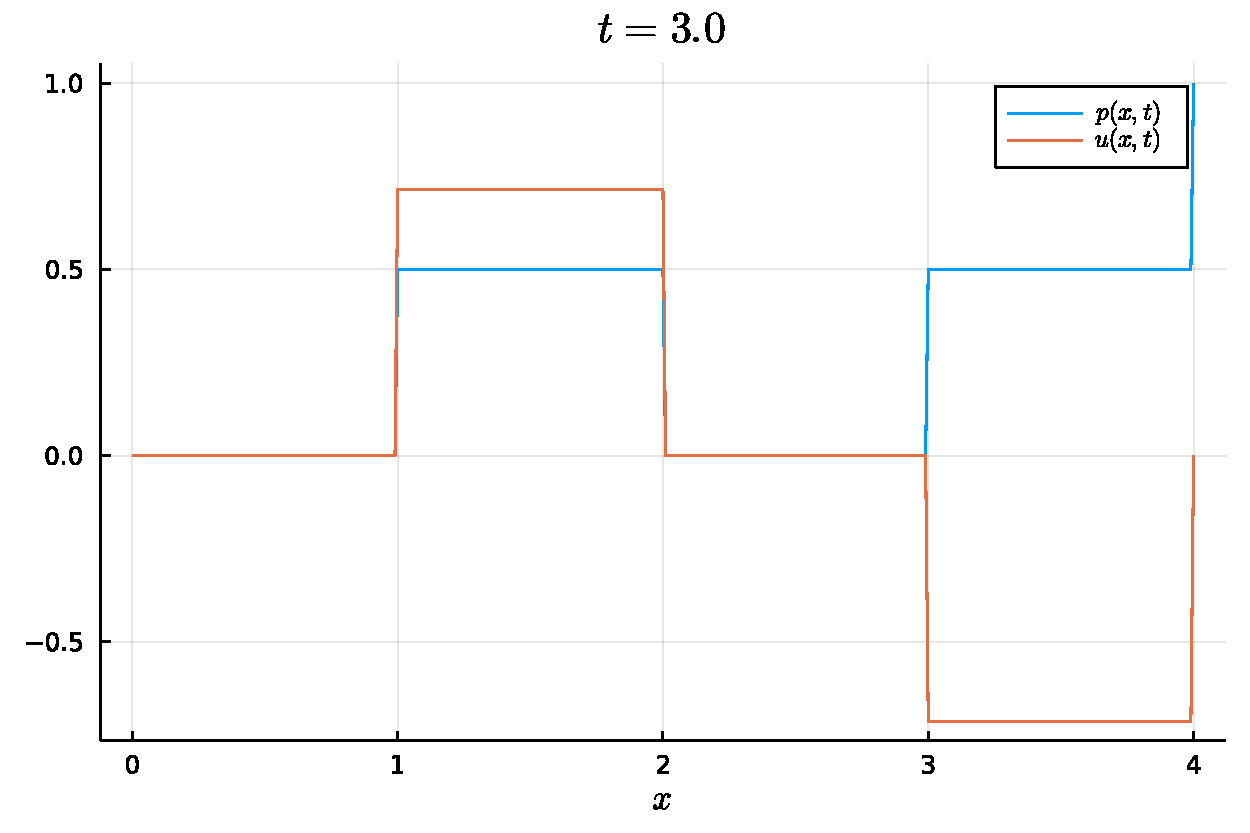
\includegraphics[width=\linewidth]{prob3-5-6.pdf}
\end{subfigure}
\end{figure}
We remark that we need to fix $c_0$ in order to obtain meaningful plots since this affects what time different states are achieved at, but these can be related to plots at any $c_0$ by taking $t\to t/c_0$. The choice of $Z_0$ matters only in the magnitude of $u(x,t)$ in regions where it is nonzero. We see a sudden spike in the plot for $t=0.5$ because it occurs exactly on a phase transition.

\section{Problem 3.8}
Consider a general hyperbolic system $q_t+Aq_x=0$ in which $\lambda=0$ is a single or multiple eigenvalue. In this case, its associated scalar problem is simply $w_t=0$ which has solution $\mathring{w}(x)$. Note that this does not have any arbitrary constants, so no boundary conditions are required\footnote{Of course, we could impose boundary conditions if we wanted to provided they were satisfied by our initial condition.}. Thus, we do not need any boundary conditions for zero eigenvalues. Combining this with our result for nonsingular $A$, if our system has $n$ negative eigenvalues, a zero eigenvalue with multiplicity $j$, and $m-n-j$ positive eigenvalues, then we need $m-n-j$ boundary conditions at the left boundary and $n$ at the right.

\section{Problem 4.2}
\subsection{Part a}
In the case where the unit CFL condition is satisfied, we note that waves propagate through the entirety of each cell exactly. We sketch this in the following analog to Figure 4.5(a).\\
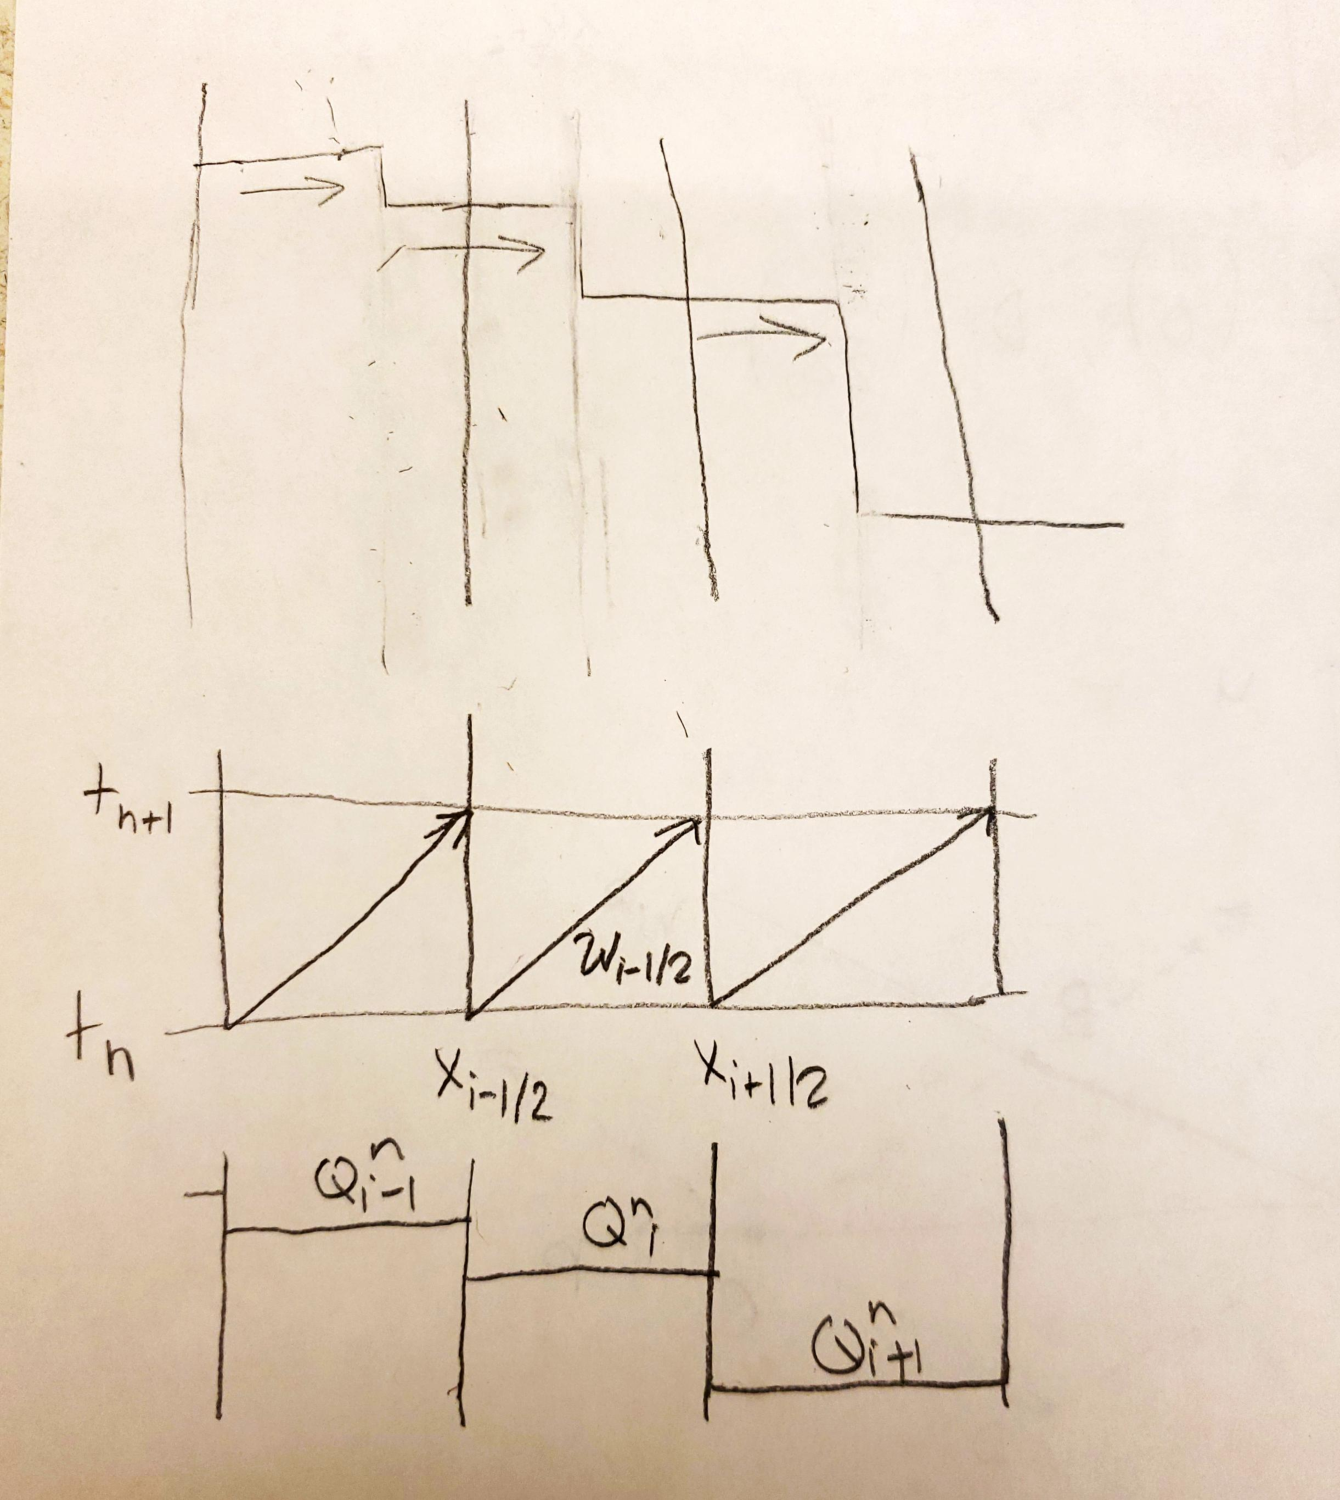
\includegraphics[scale=0.5]{574end_me.pdf}
\subsection{Part b}
Consider the Lax-Friedrichs method (4.20)
\[
Q^{n+1}_i=\half(Q^n_{i-1}+Q^n_{i+1})-\frac{\Delta t}{2\Delta x}\left(f(Q^n_{i+1})-f(Q^n_{i-1})\right)
\]
applied to the equation $q_t+\bar{u}q_x=0$. If we assume that $\bar{u}\Delta t=\Delta x$, then we have that 
\begin{align*}
Q^{n+1}_i&=\half(Q^n_{i-1}+Q^n_{i+1})-\frac{\Delta t}{2\Delta x}\left(\bar uQ^n_{i+1}-\bar uQ^n_{i-1}\right)\\&=
\half(Q^n_{i-1}+Q^n_{i+1})-\half\left(Q^n_{i+1}-Q^n_{i-1}\right)=Q^n_{i-1},
\end{align*}
so the method satisfies the unit CFL condition. If we instead consider the two-step Lax-Wendroff method under the same assumptions, we have from our previous work\footnote{This is clear by replacing $i+1$ with $i$ everywhere.} that 
\[
Q^{n+1/2}_{i-1/2}=\half(Q^n_{i-1}+Q^n_{i})-\frac{\Delta t}{2\Delta x}\left(f(Q^n_{i})-f(Q^n_{i-1})\right)=Q^n_{i-1}.
\]
Similarly, 
\[
Q^{n+1/2}_{i+1/2}=\half(Q^n_{i}+Q^n_{i+1})-\frac{\Delta t}{2\Delta x}\left(f(Q^n_{i+1})-f(Q^n_{i})\right)=Q^n_{i}.
\]
Thus, our second step becomes
\begin{align*}
Q^{n+1}_i&=Q^n_i-\frac{\Delta t}{\Delta x}\left(f\left(Q^{n+1/2}_{i+1/2}\right)-f\left(Q^{n+1/2}_{i-1/2}\right)\right)=Q^n_i-\frac{\Delta t}{\Delta x}\left(\bar uQ^n_i-\bar uQ^n_{i-1}\right)\\&=
Q^n_i-\left(Q^n_i-Q^n_{i-1}\right)=Q^n_{i-1},
\end{align*}
so the method also satisfies the unit CFL condition.
\subsection{Part c}
Now, we apply Godonov's method to the system (2.50) with $u_0=0$ with the assumption that $c_0\Delta t=\Delta x$. Then, since we know that the eigenvalues are given by $\lambda^1=-c_0$, $\lambda^2=c_0$, we find that 
\begin{align*}
Q^{n+1}_i&=Q^n_i-\frac{\Delta t}{\Delta x}\left(\sum_{p=1}^m(\lambda^p)^-\mathcal W^p_{i+1/2}+\sum_{p=1}^m(\lambda^p)^+\mathcal W^p_{i-1/2}\right)\\&=
Q^n_i-\frac{\Delta t}{\Delta x}\left(-c_0\mathcal W^1_{i+1/2}+c_0\mathcal W^2_{i-1/2}\right)=Q^n_i-\left( \mathcal W^2_{i-1/2}-\mathcal W^1_{i+1/2}\right).
\end{align*}
Now, using Mathematica, we compute
\begin{align*}
\alpha_{i-1/2}=R^{-1}\begin{pmatrix}
	p^n_{i-1}-p^n_{i}\\
	u^n_{i-1}-u^n_{i}
\end{pmatrix}=\frac{1}{2}\begin{pmatrix}
\frac{1}{Z_0}(p_{i-1}^n-p_i^n)-(u_{i-1}^n-u_i^n)\\
-\frac{1}{Z_0}(p_{i-1}^n-p_i^n)-(u_{i-1}^n-u_i^n)\\
\end{pmatrix},\\
\alpha_{i+1/2}=R^{-1}\begin{pmatrix}
	p^n_{i}-p^n_{i+1}\\
	u^n_{i}-u^n_{i+1}
\end{pmatrix}=\frac{1}{2}\begin{pmatrix}
	\frac{1}{Z_0}(p_{i}^n-p_{i+1}^n)-(u_{i}^n-u_{i+1}^n)\\
	-\frac{1}{Z_0}(p_{i}^n-p_{i+1}^n)-(u_{i}^n-u_{i+1}^n)\\
\end{pmatrix}.
\end{align*}
With this, we can use Mathematica to find that 
\begin{align*}
Q^{n+1}_n=Q^n_i-\left(\alpha^2_{i-1/2}r^2-\alpha^1_{i+1/2}r^1\right)=\frac{1}{2}\begin{pmatrix}
(p^n_{i-1}+p^n_{i+1})+Z_0(u^n_{i-1}-u^n_{i+1})\\\frac{1}{Z_0}(p^n_{i-1}-p^n_{i+1})+(u^n_{i-1}+u^n_{i+1}).
\end{pmatrix}
\end{align*}
We can see that this is the exact solution obtained from characteristic theory by letting the $(i-1)$th entry correspond to $x-c_0t$ and the $(i+1)$th entry correspond to $x+c_0t$. Then, we note that this exactly matches the general solution we obtained in problem 3.4.
\subsection{Part d}
If we consider part c in the case where $u_0\neq0$, it is not possible to obtain a similar exact result. This is because our ability to find a suitable Courant number required us being able to factor out the eigenvalues. As the eigenvalues are now given by $u_0\pm c_0$, there is now no scaling which can eliminate both.

\section{Problem 4.3}
Consider the following method for the advection equation with $\bar u>0$.
\begin{align*}
Q^{n+1}_i&=Q^n_i-(Q^n_i-Q^n_{i-1})-\left(\frac{\bar u\Delta t-\Delta x}{\Delta x}\right)(Q^n_{i-1}-Q^n_{i-2})\\&=
Q^n_{i-1}-\left(\frac{\bar u\Delta t}{\Delta x}-1\right)(Q^n_{i-1}-Q^n_{i-2}).
\end{align*}
\subsection{Part a}
We consider the case $\Delta x\leq\bar u\Delta t\leq2\Delta x$. We can see that this method results from a wave-propagation algorithm as in Figure 4.5(a) by noting that the function shifts by a distance of $\bar u\Delta t$ over time $\Delta t$. In our case, this means that our wave propagates entirely through the adjacent cell and a fraction of $\frac{\bar u\Delta t}{\Delta x}-1$ through the next. We can write this relation as
\[
Q_i^{n+1}=Q^n_i-\mathcal W_{i-1/2}+\left(\frac{\bar u\Delta t}{\Delta x}-1\right)(-\mathcal W_{i-3/2}).
\]
Using the fact that this is a scalar problem, we can replace the waves with the jumps to get
\begin{align*}
Q_i^{n+1}&=Q^n_i-(Q_i^n-Q^n_{i-1})-\left(\frac{\bar u\Delta t}{\Delta x}-1\right)(Q^n_{i-1}-Q^n_{i-2})\\&=
Q^n_{i-1}-\left(\frac{\bar u\Delta t}{\Delta x}-1\right)(Q^n_{i-1}-Q^n_{i-2})
\end{align*}
which is our method exactly.
\subsection{Part b}
If we instead wish to view our method based on linear interpolation in the realm of Figure 4.4(a), our choice of $\bar u\Delta t$ means that we need to interpolate between $Q^n_{i-1}$ and $Q^n_{i-2}$. Again noting that we are a fraction of $\frac{\bar u\Delta t}{\Delta x}-1$ through this cell, we obtain the method
\begin{align*}
Q^{n+1}_i&=\left(\frac{\bar u\Delta t}{\Delta x}-1\right)Q^n_{i-2}+\left(1-\left(\frac{\bar u\Delta t}{\Delta x}-1\right)\right)Q^n_{i-1}\\&=
Q^n_{i-1}-\left(\frac{\bar u\Delta t}{\Delta x}-1\right)(Q^n_{i-1}-Q^n_{i-2})
\end{align*}
which again is our method exactly.
\subsection{Part c}
If we take $\bar u\Delta t/\Delta x=1$, then the second term in our method drops out entirely, so we simply have that 
\[
Q^{n+1}_i=Q^n_{i-1},
\]
meaning that our method is exact. If we instead have that $\bar u\Delta t/\Delta x=2$, then our method becomes 
\begin{align*}
Q^{n+1}_i=Q^n_{i-1}-(Q^n_{i-1}-Q^n_{i-2})=Q^n_{i-2}
\end{align*}
which is still exact because our timestep now encompasses two cells.
\subsection{Part d}
To find the CFL condition, we note that $Q^{n+1}_i$ depends on $Q^n_{i-1}$ and $Q^n_{i-2}$. This means that the numerical domain of dependence of a general point $(X,T)$ is $X-\frac{2T}{r}\leq x\leq X-\frac{T}{r}$ where $r=\Delta t/\Delta x$. The domain of dependence of the true solution is $X-\bar uT$, so our CFL condition is
\[
X-\frac{2T}{r}\leq X-\bar uT\leq X-\frac{T}{r}.
\]
This can be reduced to the condition that
\[
1\leq\bar ur\leq2,
\]
so our CFL condition is given by
\[
1\leq\frac{\bar u\Delta t}{\Delta x}\leq2
\]
as expected.
\subsection{Part e}
To determine a method of this type that works if each wave propagates through more than two cells but less than three, we revisit the interpolation approach from part b which suggests that if we want this behavior, we should interpolate as
\begin{align*}
	Q^{n+1}_i&=\left(\frac{\bar u\Delta t}{\Delta x}-2\right)Q^n_{i-3}+\left(1-\left(\frac{\bar u\Delta t}{\Delta x}-2\right)\right)Q^n_{i-2}\\&=
	Q^n_{i-2}-\left(\frac{\bar u\Delta t}{\Delta x}-2\right)(Q^n_{i-2}-Q^n_{i-3})
\end{align*}
which we would use as our numerical method.

\section{Coding problem}
See the attached Jupyter notebook.
\end{document}
